\documentclass[12pt]{article}
\usepackage{../../lecture_notes}
\usepackage{../../math}
\usepackage{../../uark_colors}

\hypersetup{
  colorlinks = true,
  allcolors = ozark_mountains,
  breaklinks = true,
  bookmarksopen = true
}

\begin{document}
\begin{center}
  {\Huge\bf Midterm 1 Study Guide}
  
  \smallskip
  {\large\it ECON 4753 — University of Arkansas}

  \medskip
  {\large Prof. Kyle Butts}
\end{center}

\section*{Overview of Topics:}
\begin{enumerate}
  
  \item[1.] Bivariate Regression
  \begin{itemize}    
    \item Given a regression coefficient, how do we interpret the marginal effect
    \begin{itemize}
      \item A one unit change in $X$ is associated with a $\hat{\beta}_1$ change in $y$
      \item DO NOT use causal langauge here
    \end{itemize}

    \item Understand regressing $y$ on an indicator variable
    \begin{itemize}
      \item How do you interpret the intercept and the coefficient on the indicator variable (difference-in-means)
    \end{itemize}

    \item Regression $y$ on a set of indicator variables for each value of a discrete variable
    \begin{itemize}
      \item Know what the `omitted' category means and know the coefficients are difference-in-means
    \end{itemize}
  \end{itemize}
  
  \item[2.] Time-series
  \begin{itemize}
    \item Autocorrelation coefficient and how to calculate it (e.g. calculating $\rho_1$)
  \end{itemize}

  \item[3.] Smoothing Methods
  
  \begin{itemize}
    \item Two-sided moving average: 
    \begin{itemize}
      \item The formula to calculate: $\hat{y}_t = \sum_{k = -K}^K \frac{1}{2K+1} y_{t + k}$

      \item Why are there no forecasts on the ends of the time-series
      
      \item How does increasing the number of observations on each side change the forecasting (``smoothing'')
      
      \item What sort of time-series features does a high-level of smoothing miss out on?
    \end{itemize}

    \item Decomposition of time-series into a Trend term, Seasonality term, and remanining noise: $y_t = T_t + S_t + \varepsilon_t$
    \begin{itemize}
      \item How to estimate each part: 
      \begin{enumerate}
        \item $2 \times L$ moving average to estimate $T_t$
        \item regressing $y_t - \hat{T}_t$ on seasonal dummies to estimate $S_t$
        \item $\hat{\varepsilon}_t = y_t - \hat{T}_t - \hat{S}_t$
      \end{enumerate}

      \item How to interpret each estimate 
    \end{itemize}

    \item One-sided moving average:
    \begin{itemize}
      \item The formula to calculate: $\hat{y}_t = \sum_{k = 1}^K \frac{1}{K+1} y_{t - k}$

      \item How does increasing the number of observations included change the forecasting (``smoothing'')

      \item What sort of time-series features does a high-level of smoothing miss out on?
    \end{itemize}

    \item Simple exponential smoothing
    \begin{itemize}
      \item The formula to calculate: $\hat{y}_{t+1} = \alpha y_t + (1 - \alpha)\hat{y}_t$
      
      \item The notion of $\alpha$ and `updating' the forecast
      
      \item How the forecasting smoothness changes with the value of $\alpha \in [0, 1]$
    \end{itemize}
  \end{itemize}
  

  \item[4.] Time-series Regression
  \begin{itemize}
    \item Know the trade-off between local smoothing methods and time-series \emph{regression} models (e.g. better understanding sudden shocks vs. understanding long-term trends and seasonality)
    
    \item Estimating seasonality
    \begin{itemize}
      \item How to interpret regression table and omitted category
      
      \item Significance tests of coefficients and how to interpret them
      
      \item Comparing two month's via a coefficient test and how to set up the regression properly to do this
      
      \item Year-by-month indicators vs. Monthly indicators
    \end{itemize}

    \item Linear time-trend model
    \begin{itemize}
      \item Interpret coefficient estimate
      
      \item How to forecast with a linear time-trend
      
      \item Why should you not use higher-order polynomial terms for time-trends
    \end{itemize}

    \item Piecewise linear trends
    \begin{itemize}
      \item What is the advantage of piecewise linear trends over a single linear trend
      
      \item What are ``breakpoints''?
      
      \item Intuition on how you might select breakpoints (using the MSPE)
    \end{itemize}

    \item Indicator for ``weird shocks''
    \begin{itemize}
      \item Understand why you might include an indicator for a weird period of the time-series
    \end{itemize}
  \end{itemize}
\end{enumerate}



\newpage
\section*{Study Questions}

\subsection*{Time-series}
\begin{enumerate}
  \item Calculate the first lag autocorrelation coefficient, $\rho_1$, for the following time-series data: 
  
  $1.34, 1.78, 3.20, 4.32, 5.10, 6.24, 6.80$
\end{enumerate}

\subsection*{Smoothing Methods}
\begin{enumerate}
  \item You observe the following time-series for $t = 1, \dots, 7$. By hand calculate the two-sided moving average for $\hat{y}_4$ with $K = 2$ periods on each side
  
  $1.34, 1.78, 3.20, 4.32, 5.10, 6.24, 6.80$

  \item Why might you want to use a larger $K$ for a rolling average when the data is measured noisily (like in aggregate survey statistics)?
  
  \item Say you have a time-series on data where there are a lot of sudden jumps up or down for short periods. For this time-series, would you prefer a larger or smaller $K$ and why?
  
  \item Say you have a time-series observed every month. In words, describe (1) what seasonality is and (2) describe why a smoothing method might not capture seasonality well. You can use an example if that helps
  
  \item Say you have weekly data on the amount of movie tickets sold by AMC Theatres over the last 10 years. Think about decomposing the time-series. Describe the difference between the time-trend, $T_t$, and seasonality, $S_t$. 
  
  \item Below we present the classical decomposition of monthly jewlery sales in the US.
  \begin{center}
    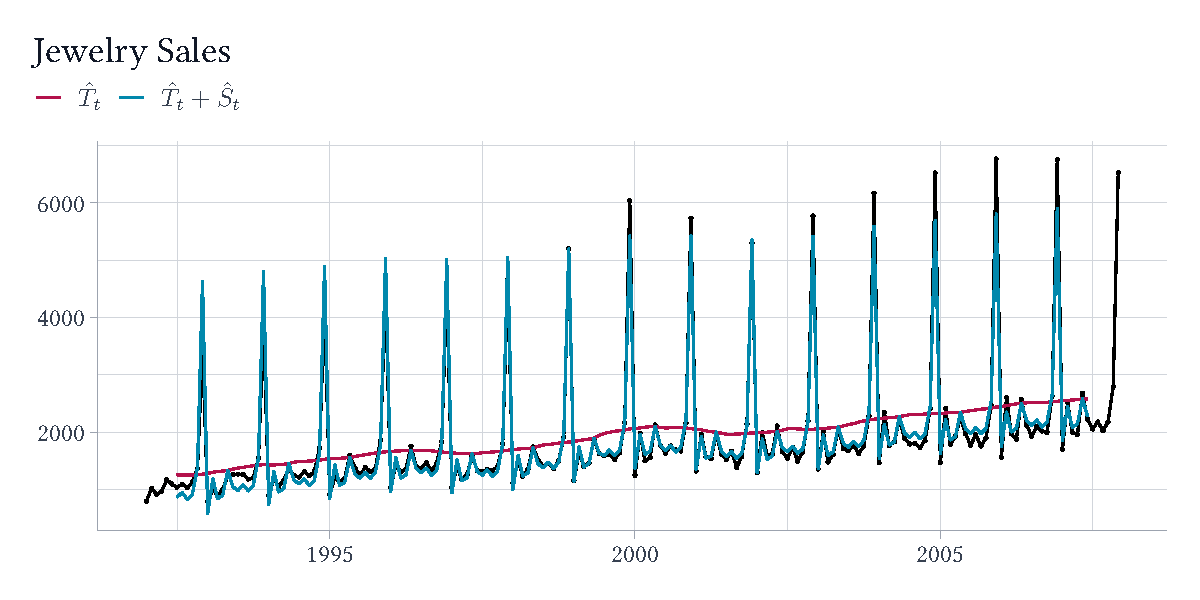
\includegraphics[width = 0.9\textwidth]{figures/jewelry_decomposition.pdf}
  \end{center}
  \begin{itemize}
    \item Why are there no estimates on the ends of the time-series?
    
    \item Would a 3-month moving average do a good job at forecasting into the future? Why or why not?
  \end{itemize}
\end{enumerate}

\subsection*{Time-series Regression}
\begin{enumerate}
  \item We present time-series regression estimates using monthly jewlery sales in the US. 

  \begin{codeblock}[{}]
OLS estimation, Dep. Var.: jewelry_sales
                  Estimate Std. Error  t value   Pr(>|t|)    
(Intercept)      1460.2500    66.2759 22.03289  < 2.2e-16 ***
quarter(date)::2  201.0208    87.7863  2.28989 2.3138e-02 *  
quarter(date)::3   86.1458    78.3546  1.09944 2.7298e-01    
quarter(date)::4 1550.4375   270.5341  5.73102 3.9133e-08 ***
---
Signif. codes:  0 '***' 0.001 '**' 0.01 '*' 0.05 '.' 0.1 ' ' 1
  \end{codeblock}

  \begin{itemize}
    \item Which quarter has the highest sales? 
    
    \item Does the 4th quarter have a significantly different sales than the 1st quarter? 
    
    \item Describe how you could modify this regression to test if quarter 2 has significantly different sales than quarter 3
  \end{itemize}


  \item Consider extending the time-series past the 2008 recession and into the 2010s
  \begin{itemize}
    \item Why might we be concerned with our time-series regression estimates when including a recession? What could a possible solution be?
  \end{itemize}

  \item Given that this data is trending, we add a linear time-trend to our jewelry sales regression

  \begin{codeblock}[{}]
OLS estimation, Dep. Var.: jewelry_sales
Standard-errors: Heteroskedasticity-robust 
                     Estimate Std. Error  t value   Pr(>|t|)    
(Intercept)      -164797.9300 27392.9818 -6.01606 9.2227e-09 ***
year(date)            83.1499    13.7020  6.06844 7.0290e-09 ***
quarter(date)::2     201.0208    48.8162  4.11791 5.7330e-05 ***
quarter(date)::3      86.1458    44.3752  1.94131 5.3724e-02 .  
quarter(date)::4    1550.4375   254.4599  6.09305 6.1837e-09 ***
---
Signif. codes:  0 '***' 0.001 '**' 0.01 '*' 0.05 '.' 0.1 ' ' 1
  \end{codeblock}

  \begin{itemize}
    \item Are sales trending? In which direction?
    
    \item What is the omitted category in this regression? 
  \end{itemize}

\end{enumerate}



\end{document}
